\section{Genus} % (fold)
\label{sec:genus}
W tej sekcji zbadamy bardzo geometryczny niezmiennik węzłów, genus.
Wyznaczenie genusu konkretnego węzła przysparza wiele trudności, jednak jest on potężnym narzędziem podczas dowodzenia twierdzeń.
Zaczniemy jednak od przyjrzenia się powierzchniom.

\begin{definition}
\index{powierzchnia}
    Powierzchnia to dwuwymiarowa podrozmaitość topologiczna $M \subseteq \R^3$, czyli obiekt wyglądający lokalnie jak płaszczyzna: każdy punkt $x \in M$ posiada otwarte otoczenie homeomorficzne z~otwartym dyskiem $\{(x,y) : x^2 + y^2 < 1\}$.
\end{definition}

Przykładami powierzchni są sfera oraz brzeg torusa, ale też koło otwarte albo pierścień $\{(x, y) \in \R^2 : 0 < a < x^2 + y^2 < b\}$.
Dwa ostatnie przykłady mają brzeg, dwa pierwsze są brzegu pozbawione (nazywamy je powierzchniami zamkniętymi).

Rozważane przez nas powierzchnie będą posiadać dodatkowo dwie cechy: ograniczoność oraz orientowalność.
Ta druga własność sprowadza się na mocy klasyfikacji powierzchni (spójna powierzchnia zamknięta jest sferą, sumą spójną torusów lub sumą spójną rzutowych (rzeczywistych) płaszczyzn) do niezawierania homeomorficznej kopii wstęgi Möbiusa.
Podane wcześniej powierzchnie są orientowalne.

\begin{definition}
\index{charakterystyka Eulera}
    Charakterystyka Eulera $\chi(M) \in \Z$ to niezmiennik
    topologiczny powierzchni $M$, którego definicji nie podamy.
    Zamiast tego wymienimy dość reguł,
    by wyznaczyć go w~interesujących nas przypadkach:
    \begin{itemize}
        \item Charakterystyka dysku to $1$.
        \item $\chi(M_1 \sqcup M_2)=\chi(M_1) + \chi(M_2)$ dla każdych powierzchni $M_1, M_2$.
        \item Dołączenie paska zmniejsza charakterystykę powierzchni o~$1$.
        \item Dołączenie dysku do całej składowej spójności brzegu powierzchni zwiększa charakterystykę o~$1$.
    \end{itemize}
\end{definition}

\begin{definition}
\index{genus}
    Genus powierzchni $M$ posiadającej $c$ składowych spójności brzegu to
    \[
        g(M) = 1 - \frac{\chi(M) + c}{2}.
    \]
\end{definition}

\begin{proposition}
    Dwie spójne, zorientowane powierzchnie są homeomorficzne wtedy i~tylko
    wtedy, gdy mają ten sam genus i~tyle samo składowych spójności brzegu.
\end{proposition}

Najważniejsze dla nas są powierzchnie Seiferta:

\begin{definition}
\index{powierzchnia!Seiferta}
    Powierzchnia Seiferta związana z~węzłem $K$ to spójna,
    orientowanlna powierzchnia zanurzona w~$\R^3$, której brzegiem jest $K$.
\end{definition}

% \begin{example}
% Powierzchnia Seiferta dla trójlistnika:
% \begin{center}
% \begin{tikzpicture}
% [scale=0.1]
%   \clip (-17,-15) rectangle (17,15);
%   \foreach \d in {0,180} {
%       \path[OBSZAR    ,rotate=\d] (-1.25,11.5)
%       .. controls (2,14) and (6,13.5) ..  (10,12)
%       .. controls (23,7) and (15,-20)  .. (3,-13)
%       -- (1.25, -11.5)
%       .. controls (4.5,-8) and (4.5,-4) .. (0,0)
%       .. controls (4,4) and (4.5,5.5) .. (-1.25,11.5);}
%   \path[TIKZ_ARCH] (0,10) .. controls (10,0) and (-10,0) .. (0,-10);
%   \foreach \d in {0,180} {
%   \path[TIKZ_ARCH, rotate=\d] (-1.5,1.5) .. controls (-6,6) and (-3,17) .. (10,12)
%   .. controls (23,7) and (15,-20)  .. (3,-13);}
% \end{tikzpicture}
% \end{center}
% \end{example}

Nie każde uszachowienie diagramu węzła prowadzi do powierzchni Seiferta:
widać to po standardowym diagramie trójlistnika.
Pomimo to prawdziwe jest następujące stwierdzenie.

\begin{proposition}[Pontriagin, Frankl 1930]
    Każdy węzeł posiada powierzchnię Seiferta.
\end{proposition}

Dowód tego faktu opiera się na bezpośredniej konstrukcji i~pochodzi od Seiferta.

\begin{proof}
    Wybierzmy diagram $D$ dla węzła oraz orientację,
    a~następnie wyprostujmy wszystkie skrzyżowania zgodnie z~ich orientacją:

    \[
    \begin{tikzpicture}[scale=0.12, baseline=-3]
        \begin{knot}[clip width=15, end tolerance=1pt,flip crossing/.list={1}]
            \strand[semithick,Latex-] (-5,5) to (5,-5);
            \strand[semithick,-Latex] (-5,-5) to (5,5);
        \end{knot}
    \end{tikzpicture}
    \quad\longrightarrow\quad
        \begin{tikzpicture}[baseline=-0.65ex, scale=0.12]
        \useasboundingbox (-5, -6) rectangle (5, 6);
        \draw[semithick,-Latex] (-4, -5) to [out=45, in=-45] (-4, 5);
        \draw[semithick,-Latex] (4, -5) to [out=135, in=-135] (4, 5);
        \end{tikzpicture}
        \quad\longleftarrow\quad
    \begin{tikzpicture}[scale=0.12, baseline=-3]
        \begin{knot}[clip width=15, end tolerance=1pt]
            \strand[semithick,Latex-] (-5,5) to (5,-5);
            \strand[semithick,-Latex] (-5,-5) to (5,5);
        \end{knot}
    \end{tikzpicture}
    \]

    Otrzymany diagram składa się teraz z~pewnej liczby zamkniętych krzywych,
    zwanych okręgami Seiferta, które wypełniamy do dysków.
    Tam, gdzie jeden okrąg leżał wewnątrz drugiego, podnosimy wewnętrzny nad zewnętrzny.
    Przy każdym skrzyżowaniu pierwotnego diagramu doklejamy skręcony pasek do obydwu dysków.

    Dyski są dwustronne, więc ich górnej stronie przypisujemy znak $+$,
    jeśli tylko brzeg jest zorientowany dodatnio i~$-$ w~przeciwnym razie.

    \begin{center}
        %\includegraphics[width=0.75\textwidth]{seifert.png}
        (brakująca grafika)
    \end{center}
\end{proof}

% \todo[inline]{graf Seiferta jest dwudzielny i~planarny}

Otrzymana powierzchnia zorientowana, $M_D$,
nie daje się łatwo wyobrazić, ale można policzyć jej genus.
Posiada bowiem dokładnie jedną składową spójności brzegu.

%\todo[inline]{Fałsz, jest to możliwe, ale muszę nauczyć się rysować kręcone paski.}

\begin{proposition}
    Niech $K$ będzie węzłem z~diagramem $D$. Wtedy $\chi(M_D) = s - n$, gdzie $n$ jest liczbą skrzyżowań $D$, zaś $s$ jest liczbą okręgów Seiferta.
\end{proposition}

\begin{proof}
    Powierzchnia $M_d$ powstaje z~sumy rozłącznej dysków (po jednym dla każdego okręgu Seiferta) przez dołączanie pasków do ich brzegów (po jednym dla każdego skrzyżowania).
\end{proof}

Uwaga: sploty też posiadają powierzchnie Seiferta, ale odwrócenie tylko jednej składowej potrafi kompletnie zmienić powierzchnię!

Skupimy się wreszcie na genusie węzła.
Do matematyki wprowadził go Seifert w~1934 roku.

\begin{definition}[3-genus]
    Niech $K$ będzie węzłem.
    Minimalny genus spośród wszystkich powierzchni Seiferta węzła $K$ nazywamy 3-genusem i oznaczamy $g$.
\end{definition}

Znalezienie 3-genusu dowolnego węzła sprawia te same trudności, co wyznaczenie jego liczby gordyjskiej.
Dowolna powierzchnia Seiferta zadaje ograniczenie z góry.
Z dołu 3-genus można szacować przy użyciu wielomianu Alexandera:

\begin{proposition}
    Niech $K$ będzie węzłem.
    Wtedy $\operatorname{span} \Delta(t) \le 2g$.
\end{proposition}

To dolne ograniczenie jest realizowane przez pewną powierzchnię Seiferta dla każdego pierwszego węzła o~co najwyżej 11 skrzyżowaniach poza siedmioma wyjątkami: 11n42, 11n67, 11n97 ($g = 2$), 11n34, 11n45, 11n73 oraz 11n152 ($g=3$).
Jeżeli nie powoduje to nieporozumień, zamiast 3-genus można pisać po prostu genus.

Czy w definicji genusu można ograniczyć się do powierzchni Seiferta, które pochodzą od algorytmu Seiferta?
Niestety, poza pewnymi wyjątkami, nie.
Zanim przekonamy się, dlaczego tak jest, zdefiniujmy jeszcze dwa niezmienniki.

\begin{definition}[genus kanoniczny]
    Niech $K$ będzie węzłem.
    Minimalny genus spośród wszystkich powierzchni Seiferta węzła $K$, które pochodzą z~algorytmu Seiferta, nazywamy genusem klasycznym i~oznaczamy $g_c$.
\end{definition}

Pod koniec lat pięćdziesiątych Crowell i~Murasugi niezależnie zauważyli, że algorytm Seiferta zastosowany do alternującego diagramu zawsze daje powierzchnię o~minimalnej powierzchni.
Ich kombinatoryczne uzasadnienie było dość zawiłe, elementarny dowód podał Gabai w \cite{gabai86}.

Dubel trójlistnika ma genus równy $1$, ale algorytm Seiferta zastosowany wobec węzła produkuje powierzchnie o genusie co najmniej $3$, jak przewiduje ograniczenie znalezione przez Mortona w \cite{morton86} jako twierdzenie 2:

\begin{proposition}
    Niech $P(v, z)$ będzie wersją wielomianu HOMFLY spełniającą zależność
    \begin{equation}
        \frac 1v P_+ - vP_- = zP_0.
    \end{equation}
    Wtedy $M = \max \deg_z P(v, z) \le 2g_c$.
\end{proposition}

Nierówność Mortona jest równością dla wielu klas węzłów, w tym alternujących (Crowell, Murasugi), jednorodnych (które stanowią uogólnienie węzłów alternujących, Crowell w \cite{cromwell89}), whiteheadowskich dubli węzłów dwumostowych (Nakamura w \cite{nakamura06}, Tripp w \cite{tripp02}) albo precli (Brittenham w \cite{brittenham07}).
Stojmenow pokazał, że staje się równością dla węzłów o co najwyżej 12 skrzyżowaniach i znalazł przykład węzła, dla którego jest ostra.

\begin{definition}[genus wolny]
    Niech $K$ będzie węzłem.
    Minimalny genus spośród powierzchni Seiferta węzła $K$, których dopełnienie w 3-sferze jest \emph{ciałem z rączkami} (handlebody, czyli ma wolną grupę podstawową), nazywamy genusem wolnym i~oznaczamy $g_f$.
\end{definition}

Dopełnienie powierzchni Seiferta jest zawsze handlebody, dlatego też mamy oczywiste nierówności $g \le g_f \le g_c$.
Morton w 1986 roku pokazał, że genus pewnych węzłów nie jest realizowany przez żaden diagram do którego stosuje się algorytm Seiferta, choćby $10_{165}$.
Patrz \cite{morton86}.
Moriah, matematyk izraelski, mniej więcej w tym samym czasie rozwiązał problem postawiony dekadę wcześniej przez Kirby'ego \cite{kirby78}: jak duża może być różnica $g_f - g$?

\begin{proposition}
    Niech $K$ będzie węzłem, $D_k(K)$ jego dublem Whiteheada z $k \neq 0$ skręceniami, zaś $B_n(K)$ to $n$-krotne nakrycie cykliczne sfery $S^3$ rozgałęzione nad węzłem $K$.
    Jeżeli ranga pierwszej grupy homologii $B_{|4k+1|}(K)$ wynosi $r$, to
    \begin{equation}
        g_f(D_k(K)) \ge \frac {2r-1} {|8k+2|}.
    \end{equation}
\end{proposition}

\begin{proof}
    Praca \cite{moriah87}.
    Dowód opiera się na chirurgii węzłów i splotów w sferze $S^3$.
\end{proof}

\begin{corollary}
    Niech $K$ bedzie sumą spójną $n$ trójlistników, połóżmy $k = -1$.
    Wtedy pierwsza grupa homologii ma rangę $r = 2n$ i~genus wolny jest nieograniczony
    \begin{equation}
        g_f(D_{-1}(3_1^n)) \ge \frac {4n-1} {6},
    \end{equation}
    podczas gdy zwykły genus to $g(D_{-1}(3_1^n)) = 1$.
\end{corollary}

\begin{proposition}
    \label{genus_one}
    Genus wykrywa niewęzły: $K$ jest niewęzłem wtedy i tylko wtedy, gdy $g(K) = 0$.
\end{proposition}

\begin{proof}
    Oto szkic dowodu.
    Jeżeli genus wynosi zero, to $K$ ma powierzchnię Seiferta o~jednej składowej brzegowej i~genusie zero.
Dysk też ma te własności, więc korzystamy z~klasyfikacji powierzchni (dysk jest powierzchnią).
\end{proof}

\begin{proposition}
\label{genus_sum}
    Jeśli $J, K$ są węzłami, to $g (J \shrap K) = g(J) + g(K)$.
\end{proposition}

\begin{proof}
    Pokażemy najpierw, że $g(J \# K) \le g(J) + g(K)$.
    Wybierzmy powierzchnie Seiferta $M_J$ oraz $M_K$ dla $J$ oraz $K$ o~minimalnym genusie.
    Suma $J \shrap K$ powstaje z~$J$ oraz $K$, podobnie jest z~powierzchniami Seiferta:
    \[
        \begin{tikzpicture}[baseline=-0.65ex,scale=0.12]
        \draw[semithick,-Latex] (-7, -5) to (-5, -5) [in=right, out=right] to (-5, 5) to (-7, 5);
        \draw[semithick,Latex-] ( 7, -5) to ( 5, -5) [in=left, out=left] to ( 5, 5) to ( 7, 5);
        \node at (-5, 0) {$J$};
        \node at (5, 0) {$K$};
        \end{tikzpicture}
        \longrightarrow
        \begin{tikzpicture}[baseline=-0.65ex,scale=0.12]
        \draw[semithick,-Latex] (-7, -5) to (-5, -5) to [out=right, in=left] (-2, -2) -- (2, -2) to [out=right, in=left] (5, -5) to (7, -5);
        \draw[semithick,Latex-] (-7, 5) to (-5,  5) to [out=right, in=left] (-2,  2) -- (2,  2) to [out=right, in=left] (5,  5) to (7, 5);
        \node at (0, -5) {$J \# K$};
        \end{tikzpicture}
        \quad\quad
        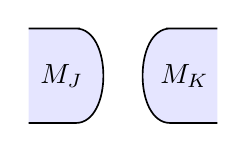
\begin{tikzpicture}[baseline=-0.65ex,scale=0.12]
        \draw[semithick,fill=blue!10!white] (-10, -5) to (-5, -5) [in=right, out=right] to (-5, 5) to (-10, 5);
        \draw[semithick,fill=blue!10!white] ( 10, -5) to ( 5, -5) [in=left, out=left] to ( 5, 5) to (10, 5);
        \node at (-6.5, 0) {$M_J$};
        \node at (6.5, 0) {$M_K$};
        \end{tikzpicture}
        \longrightarrow
        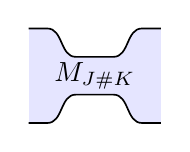
\begin{tikzpicture}[baseline=-0.65ex,scale=0.12]
        \fill[blue!10!white] (-7, -5) rectangle (7, 5);
        \draw[semithick,fill=white] (-7, -5) to (-5, -5) to [out=right, in=left] (-2, -2) -- (2, -2) to [out=right, in=left] (5, -5) to (7, -5);
        \draw[semithick,fill=white] (-7, 5) to (-5,  5) to [out=right, in=left] (-2,  2) -- (2,  2) to [out=right, in=left] (5,  5) to (7, 5);
        \node at (0, 0) {$M_{J \# K}$};
        \end{tikzpicture}
    \]

    Skoro $M_{J\#K}$ powstaje z~$M_J \sqcup M_K$ przez dołączenie paska do brzegu, mamy
    \[
        \chi(M_{J\#K}) = \chi(M_J \sqcup M_K) - 1 = \chi(M_J) + \chi(M_K)-1,
    \]
    a~przez to
    \[
        g(M_{J\#K}) = \frac{1-\chi(M_{J\#K})}{2} =
        \frac{1-\chi(M_{J})}{2} + \frac{1-\chi(M_{K})}{2}
        % = %g(M_J)+g(M_K)
        = g(J) + g(K).
    \]
    To kończy dowód pierwszej nierówności.
    Pokażemy jeszcze, że $g(J \# K) \ge g(J)+g(K)$.
    Zaczynamy od powierzchni Seiferta $M_{J\#K}$ dla $J\#K$ o~minimalnym genusie $g(M_{J\#K})$ równym $g(J\#K)$.
    Poprzez wykonanie chirurgii na powierzchni, możemy przyjąć specjalną postać jak w~poprzednim dowodzie:
    \[
        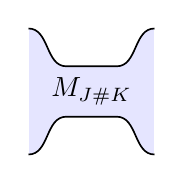
\begin{tikzpicture}[baseline=-0.65ex,scale=0.16]
            \fill[blue!10!white] (-5, -5) rectangle(5, 5);
        \draw[semithick,fill=white] (-5, -5) to [out=right, in=left] (-2, -2) -- (2, -2) to [out=right, in=left] (5, -5);
        \draw[semithick,fill=white] (-5,  5) to [out=right, in=left] (-2,  2) -- (2,  2) to [out=right, in=left] (5,  5);
            \node at (0, 0) {$M_{J \# K}$};
        \end{tikzpicture}
    \]

    Usunięcie paska daje powierzchnie Seiferta dla $M_J$ oraz $M_K$ takie, że
    \[
        g(M_J)+g(M_K)=g(M_{J\#K})=g(J\#K).
    \]
    Oznacza to, że $g(J)+g(K)\leqslant g(M_J)+g(M_K)=g(J\#K)$ i~tak naprawdę mamy równość.
\end{proof}

\begin{corollary}
\label{no_inverses}
    Jeśli suma spójna dwóch węzłów jest niewęzłem, to oba składniki także nim są.
\end{corollary}

Powrócimy teraz do węzłów pierwszych (definicja \ref{primeknot}).

\begin{proposition}
    Niech $K$ będzie węzłem.
    Jeśli $g(K) = 1$, to $K$ jest węzłem pierwszym.
\end{proposition}

\begin{proof}
    Załóżmy nie wprost, że $K = K_1 \# K_2$ jest sumą dwóch nietrywialnych węzłów.
    Z~faktu \ref{genus_sum} wynika wtedy, że $g(K) = g(K_1) + g(K_2)$.
    Zatem jeden z węzłów $K_1, K_2$ ma genus zero i jest trywialny, wbrew naszemu założeniu.
\end{proof}

Implikacja odwrotna jest fałszywa: pięciolistnik jest pierwszy, ale jego genus wynosi $2$.

\begin{proposition}
    Każdy węzeł można zapisać jako suma spójna pewnej liczby węzłów pierwszych (niewęzeł jest sumą pustej rodziny węzłów).
\end{proposition}

\begin{proof}
    Dowodzimy przez indukcję względem genusu $g(K)$.
    Przypadek bazowy $g(K) = 0$ jest oczywisty, gdyż wtedy $K$ to niewęzeł.
    Załóżmy więc, że fakt zachodzi dla węzłów $J$ genusu co najwyżej $n$.
    Niech $K$ będzie genusu $n + 1$.

    Jeśli $K$ jest pierwszy, nie ma czego dowodzić.
    W przeciwnym razie jest równoważny z~$J_1 \shrap J_2$, gdzie $J_1$ i~$J_2$ są nietrywialne.
    Mamy $g(J_1)+g(J_2)=g(K)$ oraz $g(J_1),g(J_2)\geqslant 1$.
    Zatem $g(J_1),g(J_2)\leqslant n$.
    Na mocy hipotezy indukcyjnej, $J_1$ oraz $J_2$ są równoważne sumom
    \[
        J_1 \cong K_1\#\cdots\# K_s,\qquad
        J_2 \cong K_{s+1}\#\cdots\# K_r,
    \]
    gdzie $K_i$ są pierwsze.
    Zatem $K$ jest równoważny z~$K_1\#\cdots\# K_r$, co kończy dowód.
\end{proof}

\begin{proposition}
\label{infty_primes}
    Istnieje nieskończenie wiele węzłów pierwszych.
\end{proposition}

\begin{proof}
    Pokażemy, że wszystkie węzły $(2n+2)_1$ są pierwsze, gdzie $n \ge 1$.
    Istotnie, algorytm Seiferta zastosowany do diagramu tego węzła wyprodukuje $2n+1$ okręgów.
    \[
        \begin{tikzpicture}[baseline=-0.65ex,scale=0.055]
        \begin{knot}[clip width=10, flip crossing/.list={1,4,5},end tolerance=1pt]
            \node at (0,10) {$\cdots$};
            \strand[semithick] (-30, -5) -- (-5, -5);
            \strand[semithick,-Latex]  (5, -5) -- (30, -5);
            \strand[semithick,Latex-]  (-30,-15) -- (-5,-15);
            \strand[semithick,Latex-]  (5,-15) -- (30,-15);

            \strand[semithick,domain=-90:90] plot ({7.5*cos(\x)-5}, {5*sin(\x)-10});
            \strand[semithick,domain=90:270] plot ({7.5*cos(\x)+5}, {5*sin(\x)-10});

            % zewnętrzne obręcze -- lewa strona
            \strand[semithick] (-30, 15) to [out=left, in=up]   (-45, 0);
            \strand[semithick] (-30,-15) to [out=left, in=down] (-45, 0);
            \strand[semithick] (-30,  5) to [out=left, in=up]   (-35, 0);
            \strand[semithick] (-30, -5) to [out=left, in=down] (-35, 0);

            % zewnętrzne obręcze -- prawastrona
            \strand[semithick] (30, 15) to [out=right, in=up]   (45,0);
            \strand[semithick] (30,-15) to [out=right, in=down] (45,0);
            \strand[semithick] (30,  5) to [out=right, in=up]   (35,0);
            \strand[semithick] (30, -5) to [out=right, in=down] (35,0);

            % jak w~drugim ruchu Reidemeistera - lewe
            \strand[semithick] (-30, 15) .. controls (-24, 15) and (-24,  5) .. (-20,  5);
            \strand[semithick] (-30,  5) .. controls (-24,  5) and (-24, 15) .. (-20, 15);
            \strand[semithick] (-10, 15) .. controls (-16, 15) and (-16,  5) .. (-20,  5);
            \strand[semithick] (-10,  5) .. controls (-16,  5) and (-16, 15) .. (-20, 15);

            % jak w~drugim ruchu Reidemeistera - prawe
            \strand[semithick] (30, 15) .. controls (24, 15) and (24,  5) .. (20,  5);
            \strand[semithick] (10, 15) .. controls (16, 15) and (16,  5) .. (20,  5);
            \strand[semithick] (30,  5) .. controls (24,  5) and (24, 15) .. (20, 15);
            \strand[semithick] (10,  5) .. controls (16,  5) and (16, 15) .. (20, 15);
        \end{knot}
        \end{tikzpicture}
        \longrightarrow
        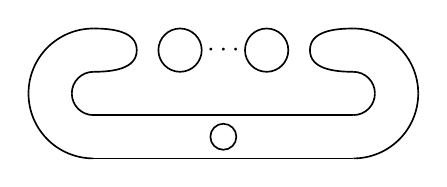
\begin{tikzpicture}[baseline=-0.65ex,scale=0.055]
            \node at (0,10) {$\cdots$};
            \draw[semithick] (-30,  -5) -- (30, -5);
            \draw[semithick] (-30, -15) -- (30,-15);

            \draw[semithick] (0,-10) circle (3);

                % zewnętrzne obręcze -- lewa strona
            \draw[semithick] (-30, 15) to [out=left, in=up]   (-45, 0);
            \draw[semithick] (-30,-15) to [out=left, in=down] (-45, 0);
            \draw[semithick] (-30,  5) to [out=left, in=up]   (-35, 0);
            \draw[semithick] (-30, -5) to [out=left, in=down] (-35, 0);

                % zewnętrzne obręcze -- prawastrona
            \draw[semithick] (30, 15) to [out=right, in=up]   (45,0);
            \draw[semithick] (30,-15) to [out=right, in=down] (45,0);
            \draw[semithick] (30,  5) to [out=right, in=up]   (35,0);
            \draw[semithick] (30, -5) to [out=right, in=down] (35,0);

            \draw[semithick] (-30, 15) to [out=right, in=up] (-20,10);
            \draw[semithick] (-30,  5) to [out=right, in=down] (-20,10);

            \draw[semithick] (30, 15) to [out=left, in=up] (20,10);
            \draw[semithick] (30,  5) to [out=left, in=down] (20,10);

            \draw[semithick] (-10, 10) circle (5);
            \draw[semithick] (10,  10) circle (5);
        \end{tikzpicture}
    \]
    Wynika stąd, że genus wynosi $\frac 12 (1 - (1+2n) + (2+2n)) = 1$, ponieważ wyznacznik ma wartość $4n+1$,
    węzły $2n+2)_1$ nie są trywialne i~są parami różne.
\end{proof}

\begin{proposition}
    Genus węzła $K$ jest związany z~wielomianem Alexandera oraz liczbą skrzyżowań:
    \[
        c(K) \ge 2 g(K) \ge \operatorname{Span}(\Delta_K(t)),
    \]
    przy czym (między innymi) dla węzłów o~co najwyżej 10 skrzyżowaniach mamy nawet równość po prawej stronie.
\end{proposition}

\index{homologia!Floera}
Wielomian Alexandera uogólnia się do (skomplikowanej) homologii Floera, pozwala ona dokładniej szacować genus węzła.

\index{węzeł!rozwłókniony}
Wspomnijmy jeszcze krótko o~specjalnym rodzaju węzłów.
Mówimy, że węzeł $K \subseteq S^3$ jest rozwłókniony\footnote{fibered}, jeśli istnieje rodzina $F_t$ powierzchni Seiferta dla $K$ sparametryzowana przez $t \in S^1$ taka, że $F_t \cap F_s = K$ dla $t \neq s$.
Dawniej nazywano je węzłami Neuwirtha.

Niewęzeł, trójlistnik i~ósemka są rozwłóknione.
Pierwszy i~ostatni współczynnik wielomianu Alexandera węzła rozwłóknionego to $\pm 1$.
Wielomianem węzła skręconego z~$q$ półskrętami jest $\Delta_q = qt - (2q+1)+q/t$, więc nie jest on rozwłókniony (dla $q \neq 1$).

% Węzeł jest rozwłókniony dokładnie wtedy, gdy stanowi grzbiet pewnego 'open book decomposition' $S^3$.

% Koniec sekcji Genus

\section{Macierz Seiferta} % (fold)
Niech $K$ będzie węzłem z powierzchnią Seiferta $S$.
Macierz Seiferta $M$ zdefiniowana jest następująco:
\[
	m_{i,j} = \operatorname{lk}(x_i, x_j^*),
\]
gdzie łuki $x_1, x_2, \ldots, x_m$ są generatorami grupy podstawowej $\pi_1(S)$, zaś gwiazdka oznacza dodatnie wypchnięcie.

Pozwala na zdefiniowanie różnych, znanych nam już niezmienników.
I tak, sygnatura węzła $\sigma(K)$ to sygnatura macierzy $M + M^t$, wyznacznik węzła to $|\det(M+M^t)|$, zaś wielomian Alexandera to $t^{-k/2}\det(M - tM^t)$, gdzie $k$ to rząd macierzy $M$.
To dopiero zalążek, więcej informacji zawiera sekcja 5.3 w podręczniku Murasugiego \cite{murasugi96}.

Trotter pokazał w 1962, że macierz Seiferta modulo $S$-równoważność stanowi niezmiennik węzłów (\cite{trotter62}).

\subsection{Sygnatura} % (fold)
\label{sub:signature}
\index{sygnatura}
Sygnatura pojawia się w~fakcie \ref{slice_signature}.

\begin{definition}
    Sygnatura to niezmiennik topologiczny zadany (kłębiastą) relacją rekurencyjną:
    \begin{itemize}[leftmargin=*]
    \itemsep0em
        \item $\sigma (\LittleUnknot) = 0$,
        \item $\sigma (K_+) - \sigma (K_-) \in \{0, 2\}$,
        \item $4 \mid \sigma (K)$ wtedy i~tylko wtedy, gdy $\nabla(2i) > 0$ (wielomian Conwaya).
    \end{itemize}
\end{definition}

\begin{proposition} \label{prop_sigma_inverse}
    Mamy $\sigma(K^*) = -\sigma(K)$ oraz $\sigma(-K) = \sigma(K)$.
\end{proposition}

\begin{proof}
    To jest twierdzenie 6.4.5 z podręcznika \cite{murasugi96}.
\end{proof}

\begin{proposition} \label{prop_sigma_additive}
    Sygnatura jest addytywna: $\sigma(K_1 \shrap \ldots \shrap K_n) = \sum_{k=1}^n \sigma(K_k)$.
\end{proposition}

Węzły achiralne mają zerową sygnaturę, zatem trójlistnik nie jest achiralny.
Z faktów \ref{prop_sigma_inverse} oraz \ref{prop_sigma_additive} wynika, że suma tak samo skręconych trójlistników nie jest achiralna ($\sigma = \pm 4$), natomiast węzeł prosty (suma różnie skręconych) ma zerową sygnaturę i jak można przekonać się ze standardowego diagramu, jest achiralny.

Sygnatura pozwala uzyskać proste oszacowanie liczby gordyjskiej od dołu:

\begin{proposition}
    Mamy $2 u(K) \ge |\sigma(K)|$.
\end{proposition}

\begin{proof}
    To jest twierdzenie 6.4.8 z podręcznika \cite{murasugi96}.
\end{proof}

Nie istnieje bezpośredni związek między sygnaturą i~liczbą mostową.
Węzeł torusowy $T_{2,n}$ jest dwumostowy, jego sygnatura wynosi $n - 1$.
Suma spójna węzłów prostych ma zerową sygnaturę i~nieograniczoną liczbę mostową.
Wynika to z~ogólniejszego faktu:

Czy istnieje węzeł o~sygnaturze $4$ i~wyznaczniku postaci $n = 4k + 1$ dla $k$ całkowitego dodatniego?
Stojmenow twierdzi, że jeśli tak jest, to wszystkie pierwsze dzielniki $n$ dają resztę $1$ z~dzielenia przez $24$ i~są większe od $2857$.

% Koniec podsekcji Sygnatura
